\section{Silicano}

\begin{frame}{Silicano}
    \begin{figure}[H]
        \centering
        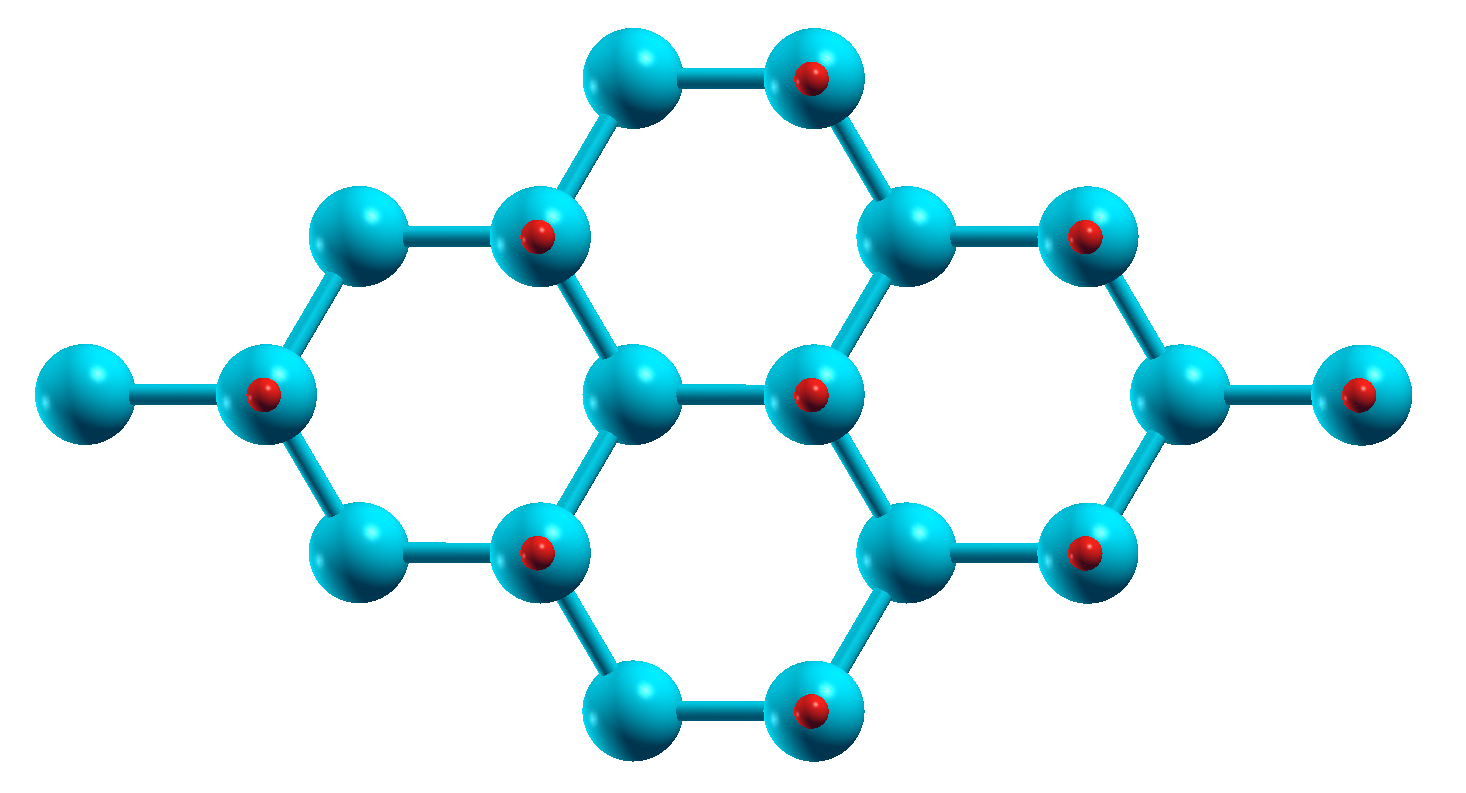
\includegraphics[scale=0.2]{images_silicano/silicano_structure.png}
        \caption{Estructura cristalina del Siliceno obtenida del archivo input con Xcrysden [Celda primitiva]}
    \end{figure}
\end{frame}

\begin{frame}
    \textbf{Parámetro de red}
    \begin{figure}[H]
        \centering
        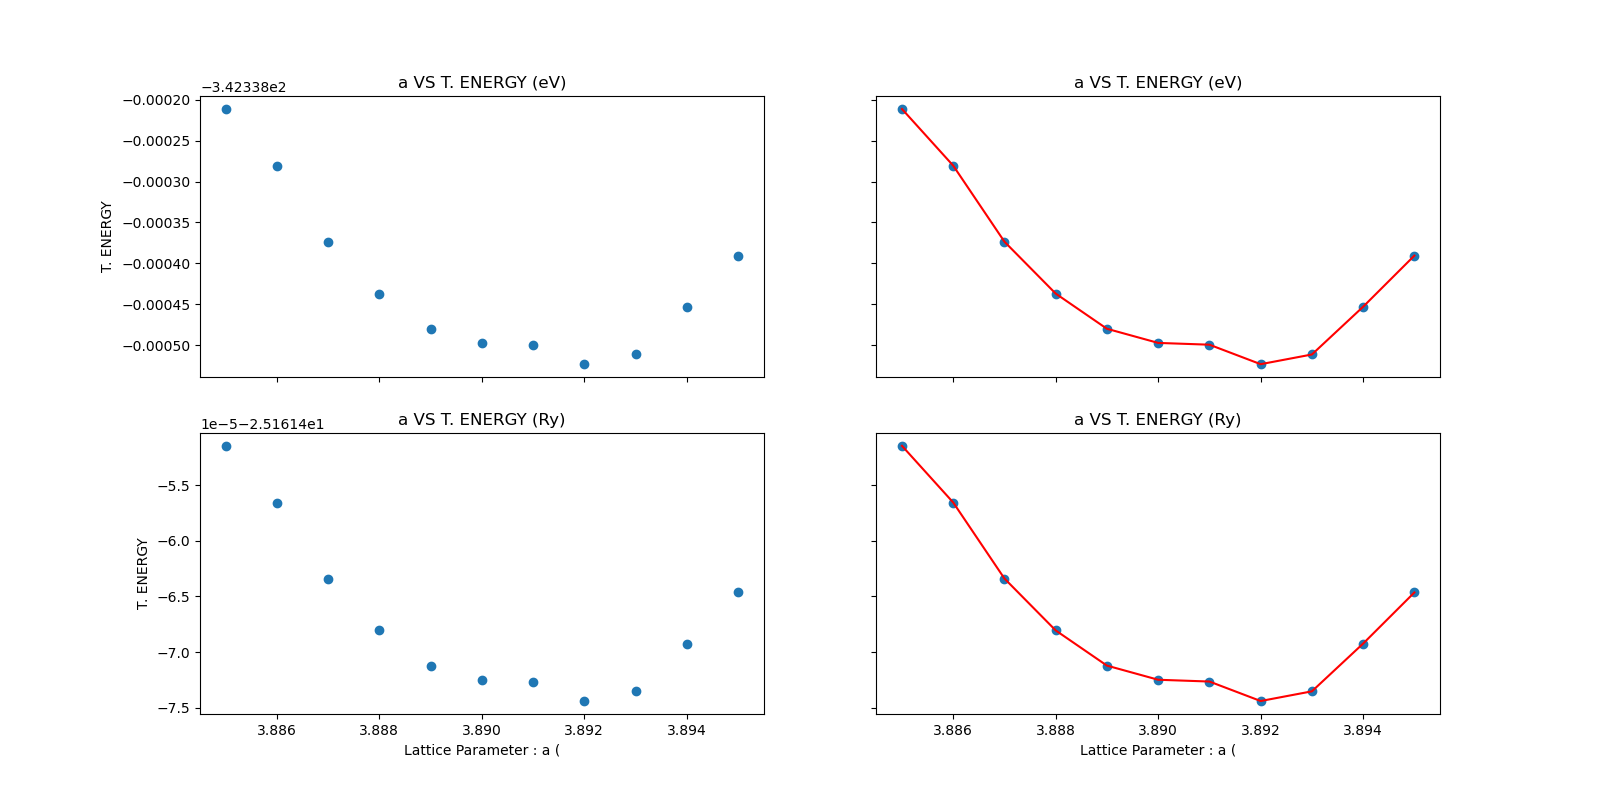
\includegraphics[scale=0.2]{images_silicano/Lattice_parameter_vs_Energy_third.png}
        \caption{Gráfica que nos muestra la energía total del sistema contra la variación del parámetro red, nos centramos en el intervalo [3.885, 3.895]}
    \end{figure}
    \noindent
    Observación: La energía se minimiza cuando el parámetro de red toma el valor de 3.92.
\end{frame}

\begin{frame}
    \textbf{Estructura electrónica de bandas}
    \begin{figure}[H]
        \centering
        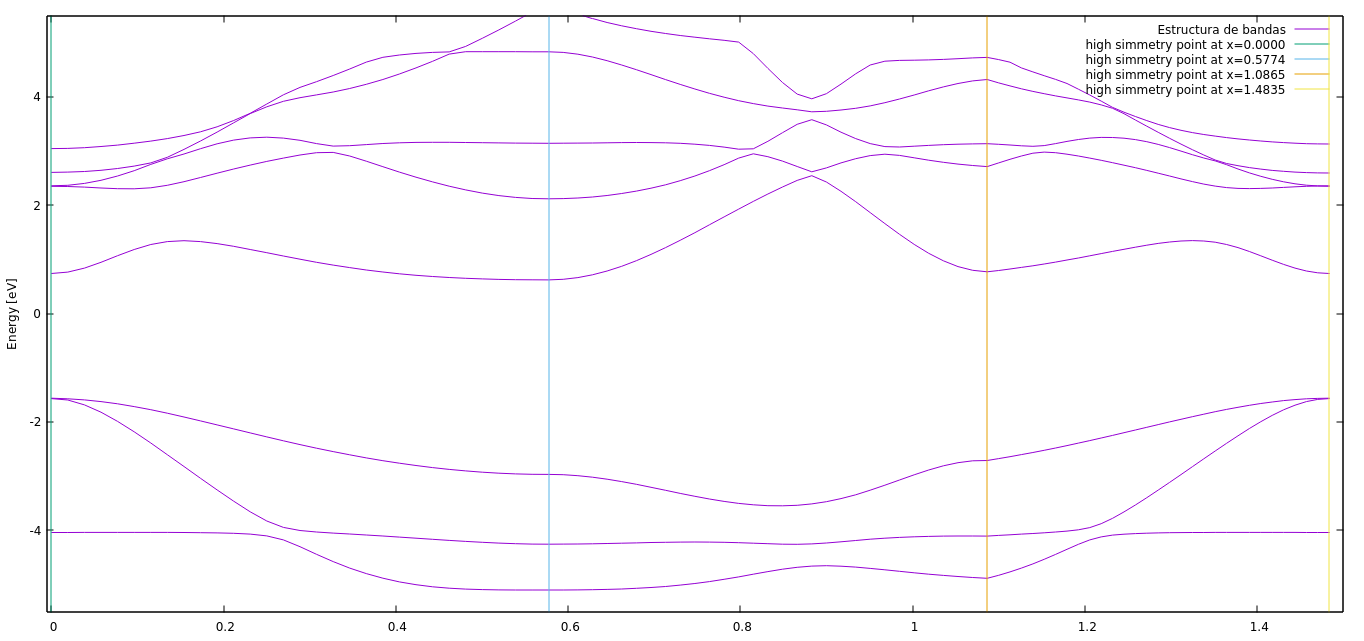
\includegraphics[scale=0.3]{images_silicano/bands_structure_silicane_10_bands_relax.png}
        \caption{Gráfica que nos muestra la estructura de bandas del siliceno, cuyo cálculo fue elaborado por cuenta propia}
    \end{figure}
\end{frame}

\begin{frame}
    \begin{figure}[H]
        \centering
        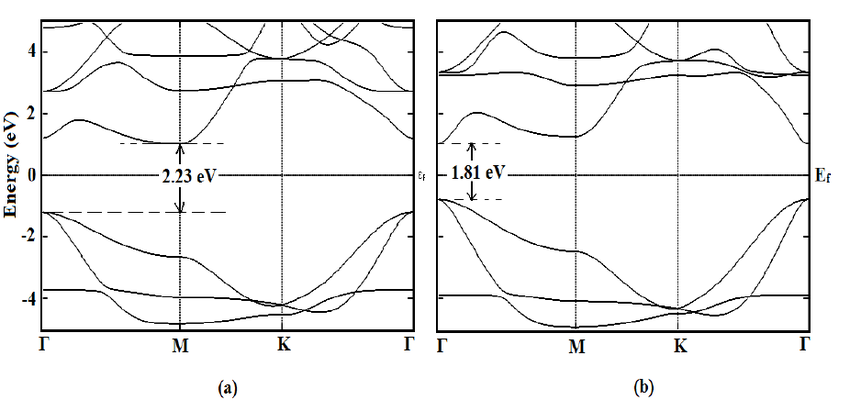
\includegraphics[scale=0.35]{images_silicano/Bandstructure-of-a-silicane-and-b-germanane.png}
        \caption{Gráfica que nos muestra la estructura de bandas del silicano [a)Siliceno y b) germanecio] }
    \end{figure}
\end{frame}



\begin{frame}
    \textbf{Densidad de estados (sin considerar el spin)}
    \begin{figure}[H]
        \centering
        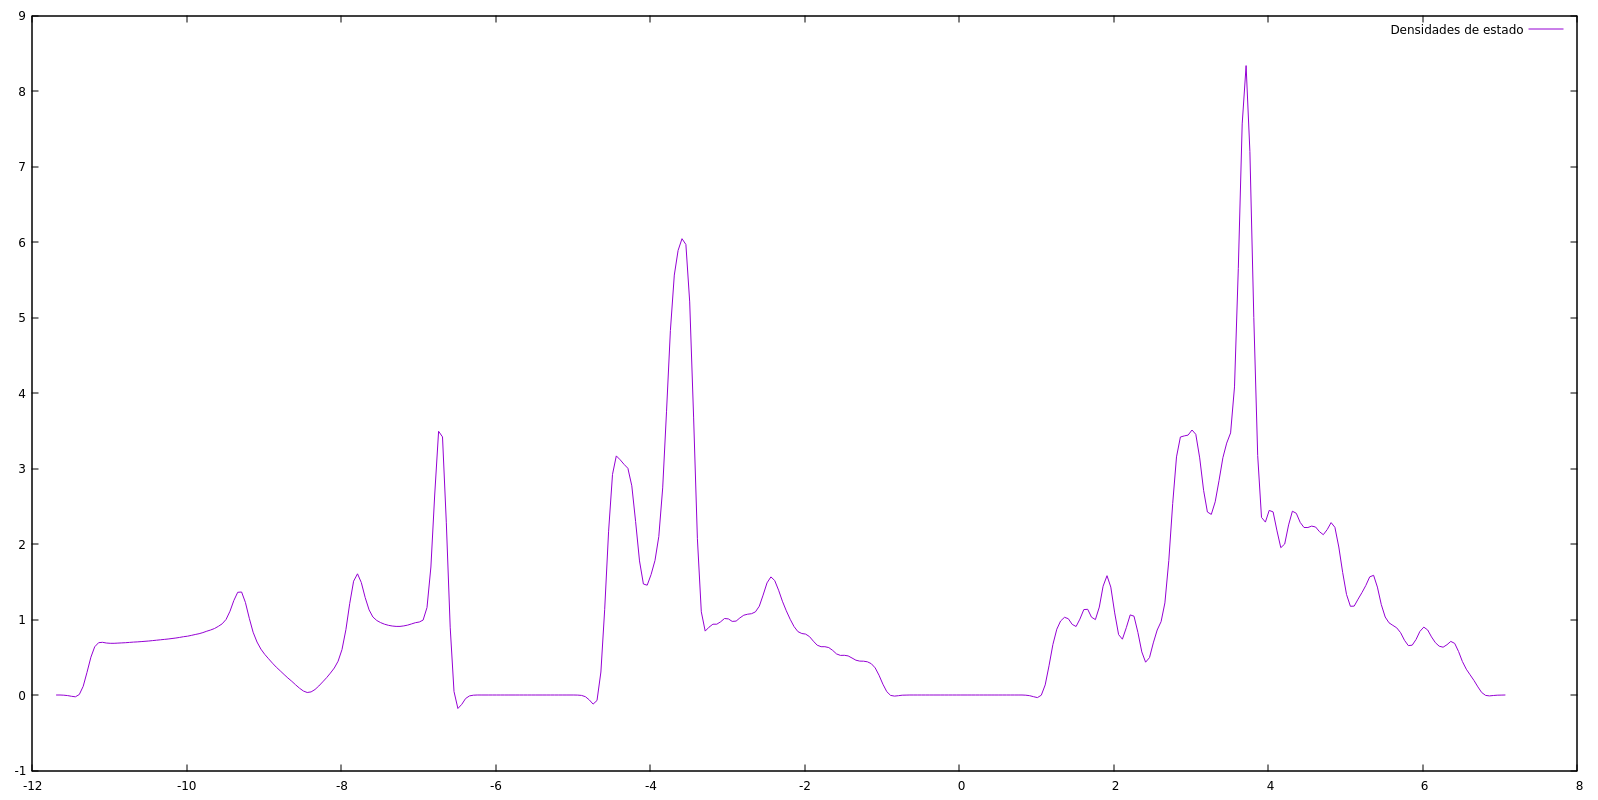
\includegraphics[scale=0.25]{images_silicano/Densidades_estado_sin_spin.png}
        \caption{Gráfica que nos muestra la densidad de estados del siliceno, sin considerar el spin.}
    \end{figure}
\end{frame}


\begin{frame}
    \textbf{Densidad de estados por nivel órbital (sin considerar el spin)}
    \begin{figure}[H]
        \centering
        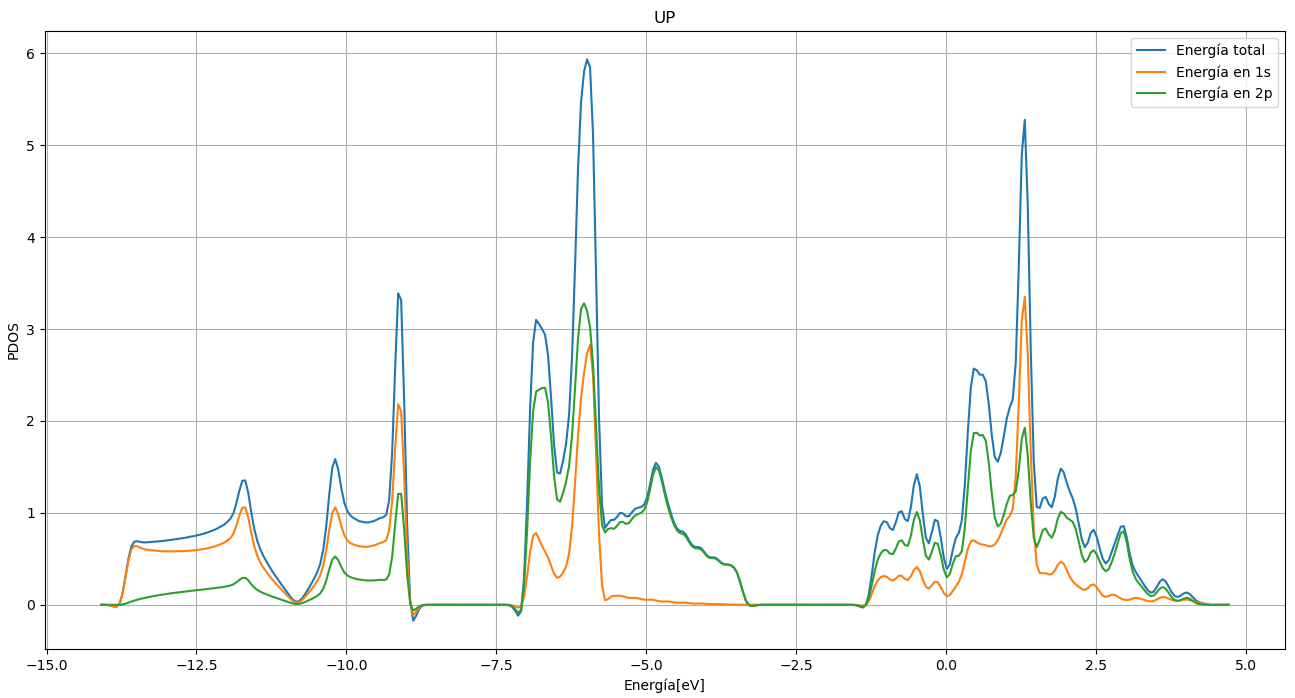
\includegraphics[scale=0.25]{images_silicano/Densidad_estados_sin_spin_up.png}
        \caption{Gráfica que nos muestra la densidad de estados en los orbitales del silicano, sin considerar el spin. [UP]}
    \end{figure}
\end{frame}

\begin{frame}
    \begin{figure}[H]
        \centering
        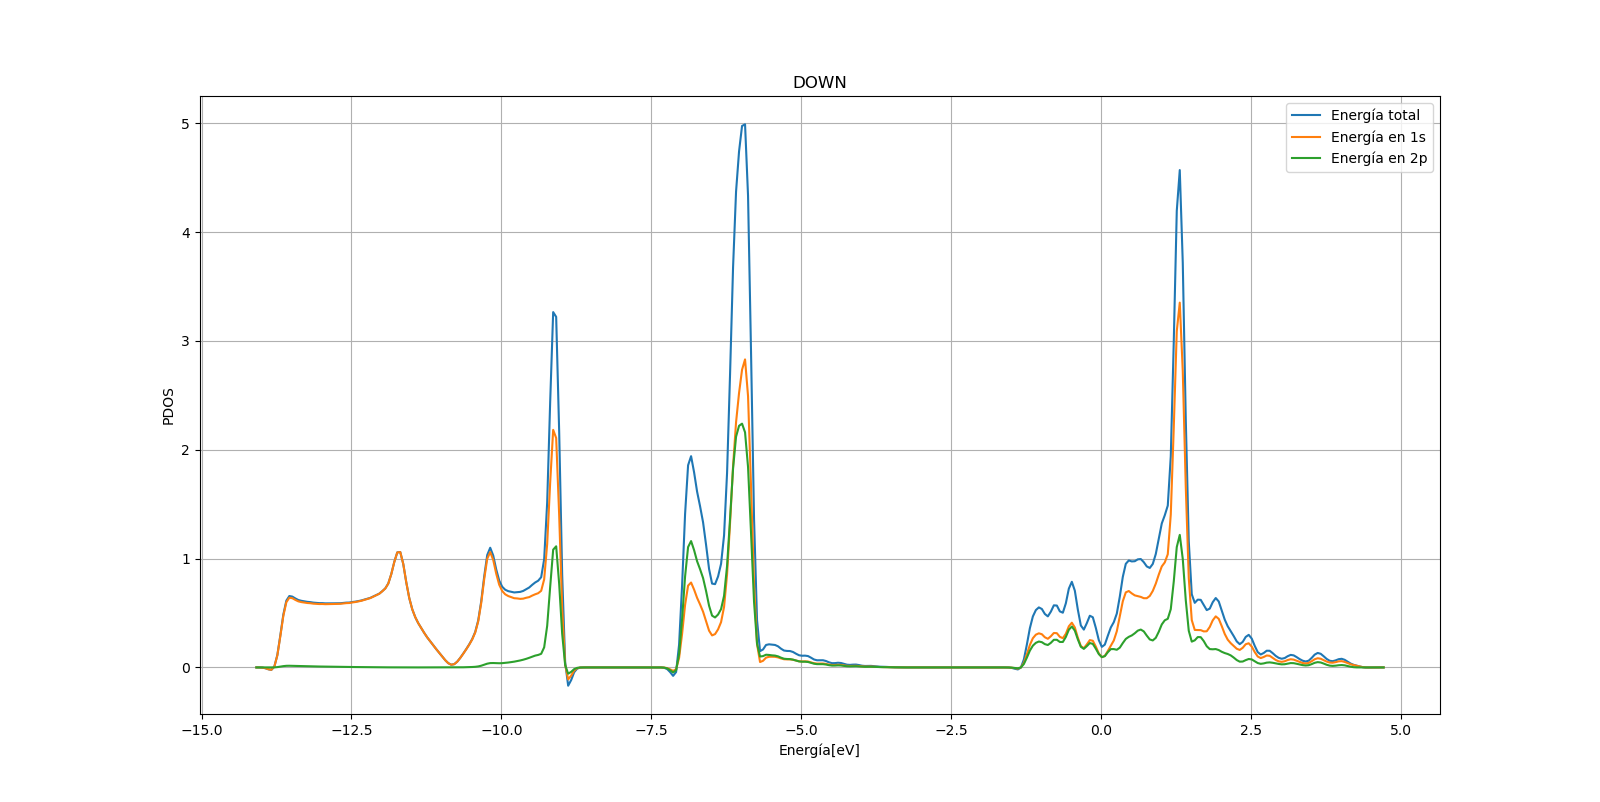
\includegraphics[scale=0.3]{images_silicano/Densidad_estados_sin_spin_down.png}
        \caption{Gráfica que nos muestra la densidad de estados en los orbitales del silicano, sin considerar el spin. [DOWN]}
    \end{figure}
\end{frame}

\vspace{0.5cm}

\begin{frame}
    \textbf{Densidad de estados por elemento(sin considerar el spin)}
    \begin{figure}[H]
        \centering
        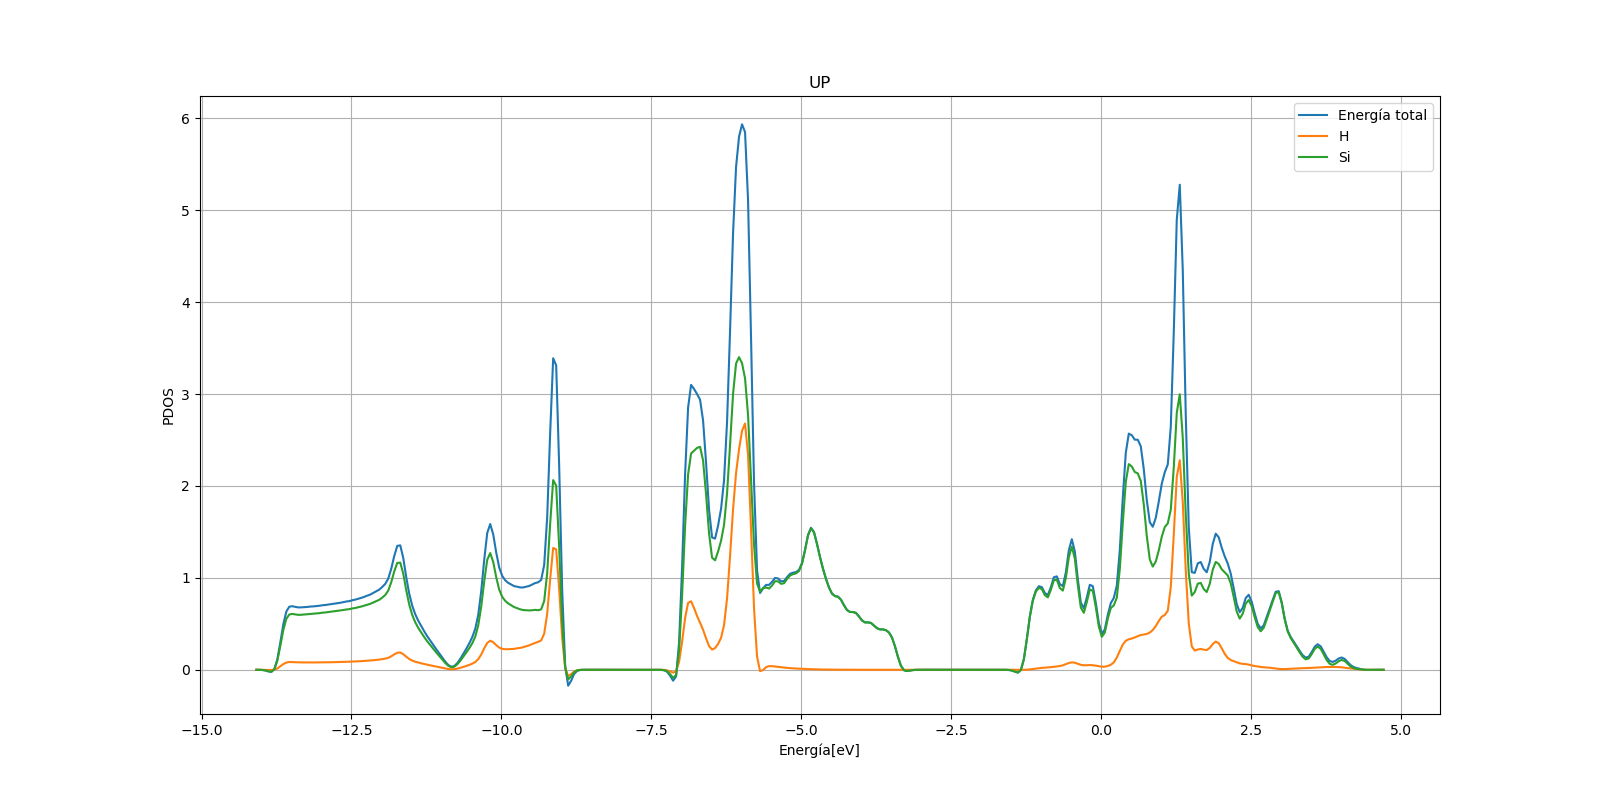
\includegraphics[scale=0.3]{images_silicano/Densidad_estados_sin_spin_up_elementos.png}
        \caption{Gráfica que nos muestra la densidad de estados por elemento, sin considerar el spin. [UP]}
    \end{figure}
\end{frame}

\begin{frame}
    \begin{figure}[H]
        \centering
        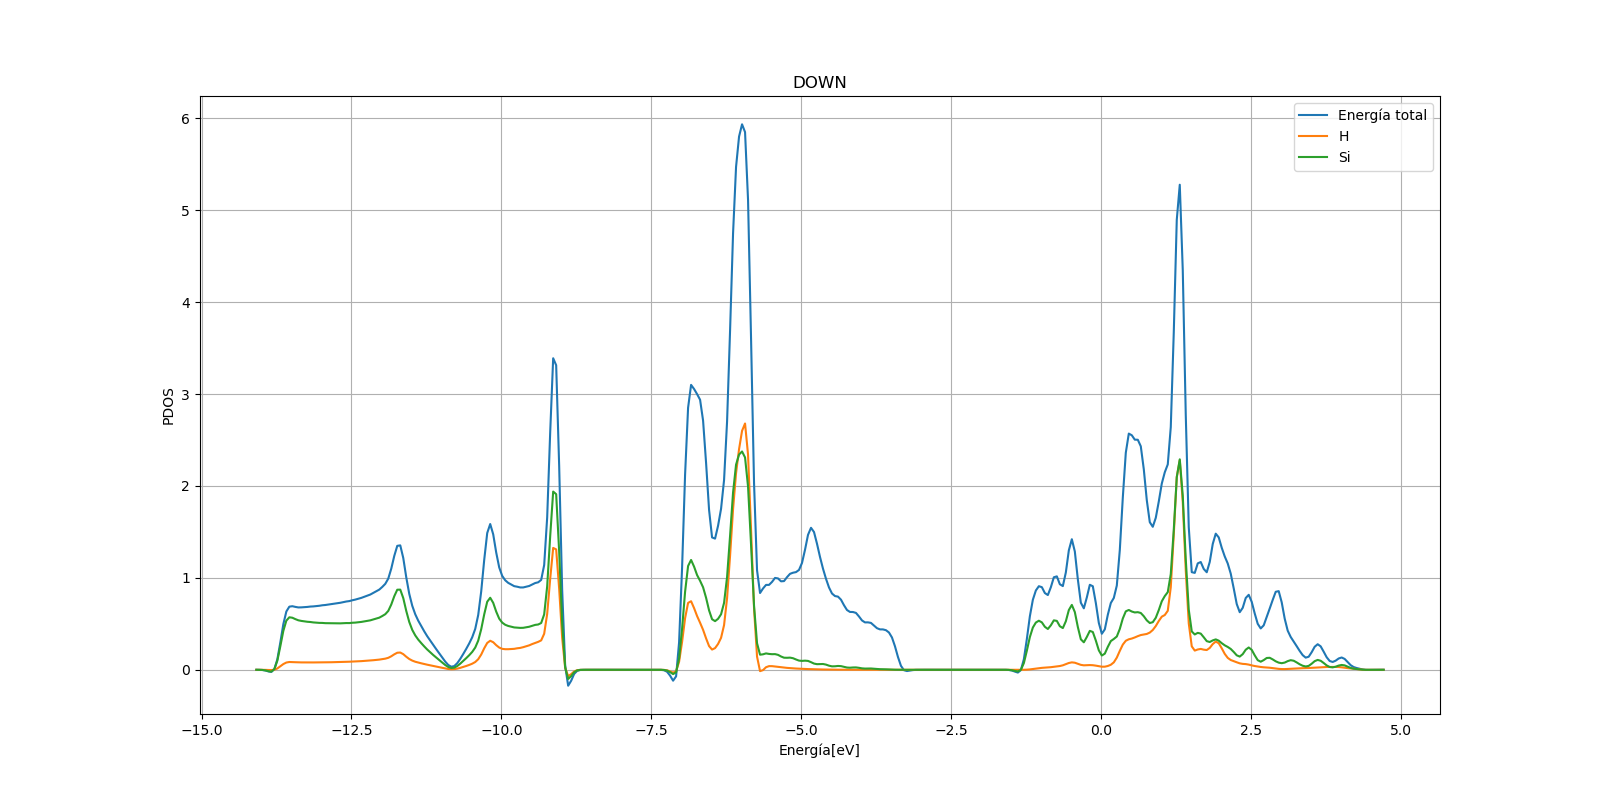
\includegraphics[scale=0.3]{images_silicano/Densidad_estados_sin_spin_down_elementos.png}
        \caption{Gráfica que nos muestra la densidad de estados por elemento, sin considerar el spin. [DOWN]}
    \end{figure}    
\end{frame}



\begin{frame}
    \textbf{Densidad de estados }
    \begin{figure}[H]
        \centering
        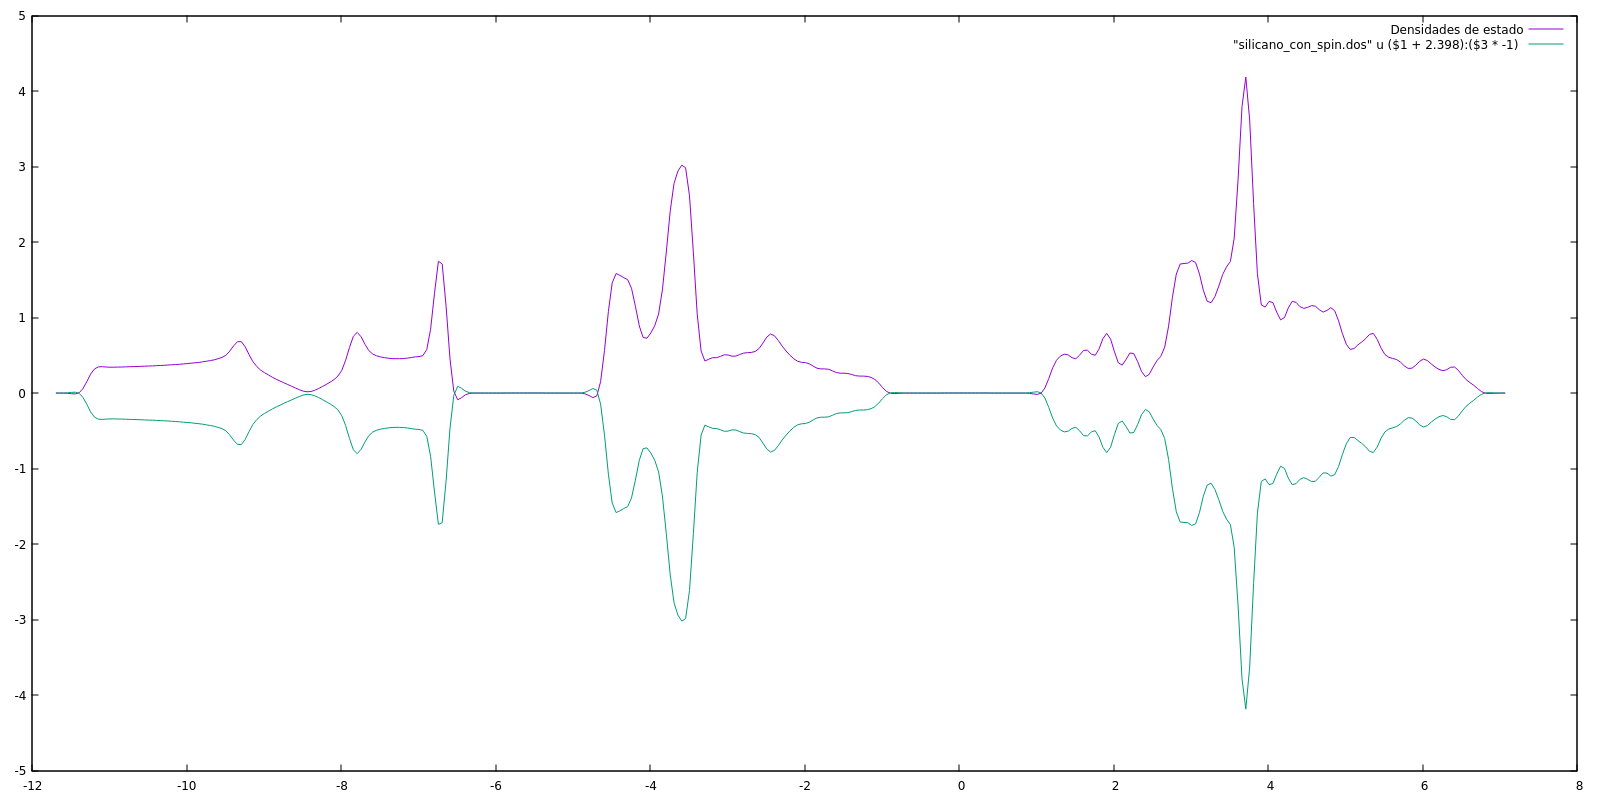
\includegraphics[scale=0.25]{images_silicano/Densidad_estados_con_spin.png}
        \caption{Gráfica que nos muestra la densidad de estados del siliceno, sin considerar el spin.}
    \end{figure}
\end{frame}


\begin{frame}
    \textbf{Densidad de estados por nivel órbital}
    \begin{figure}[H]
        \centering
        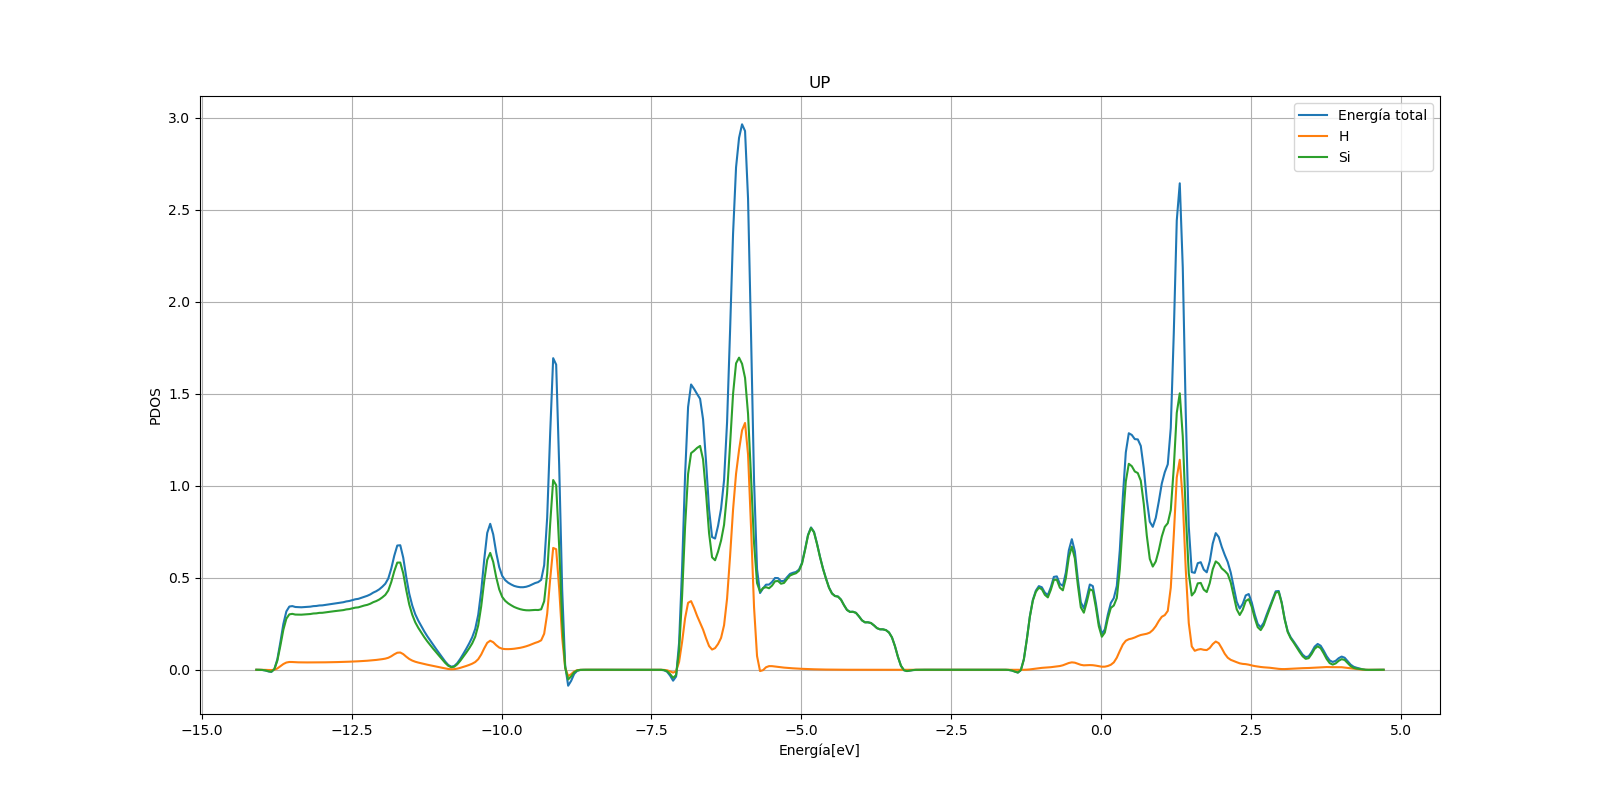
\includegraphics[scale=0.3]{images_silicano/Densidad_estados_con_spin_up_elementos.png}
        \caption{Gráfica que nos muestra la densidad de estados en los orbitales del silicano, sin considerar el spin. [UP]}
    \end{figure}
\end{frame}

\begin{frame}
    \begin{figure}[H]
        \centering
        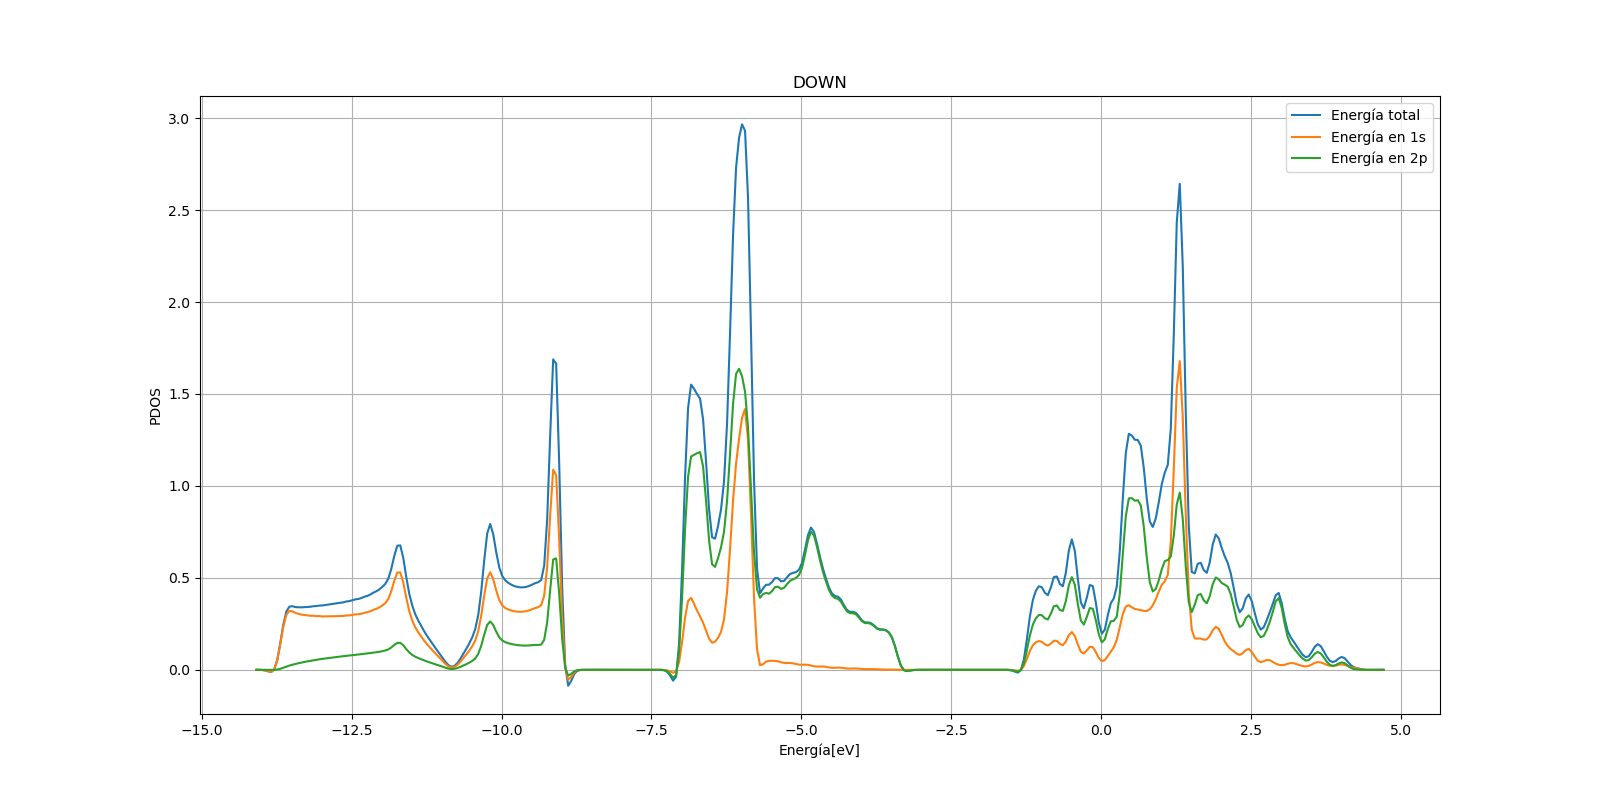
\includegraphics[scale=0.3]{images_silicano/Densidad_estados_con_spin_down.png}
        \caption{Gráfica que nos muestra la densidad de estados en los orbitales del silicano, sin considerar el spin. [DOWN]}
    \end{figure}
\end{frame}

\vspace{0.5cm}

\begin{frame}
    \textbf{Densidad de estados por elemento}
    \begin{figure}[H]
        \centering
        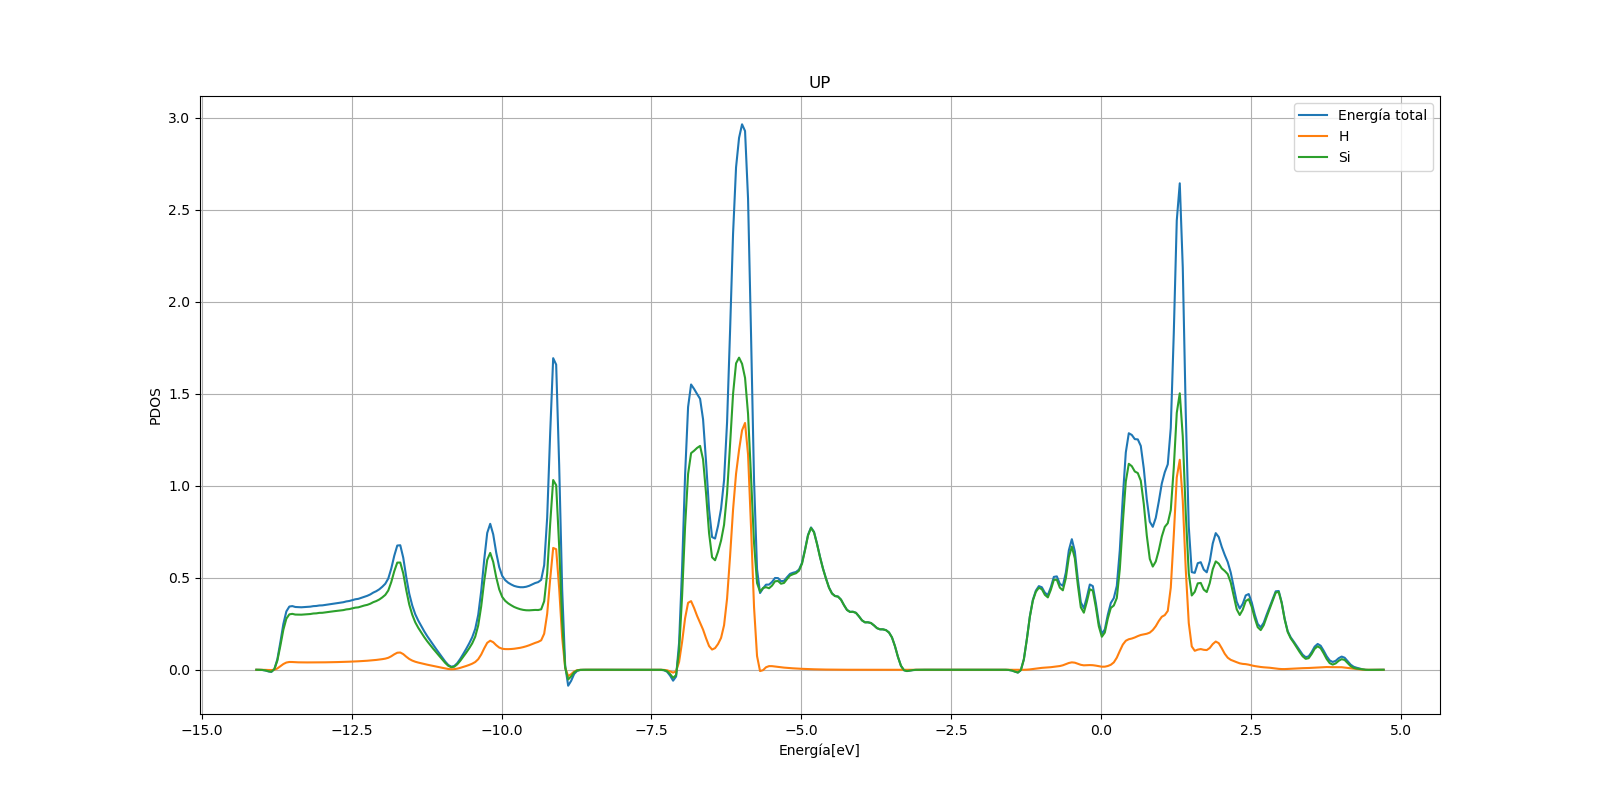
\includegraphics[scale=0.3]{images_silicano/Densidad_estados_con_spin_up_elementos.png}
        \caption{Gráfica que nos muestra la densidad de estados por elemento, sin considerar el spin. [UP]}
    \end{figure}
\end{frame}

\begin{frame}
    \begin{figure}[H]
        \centering
        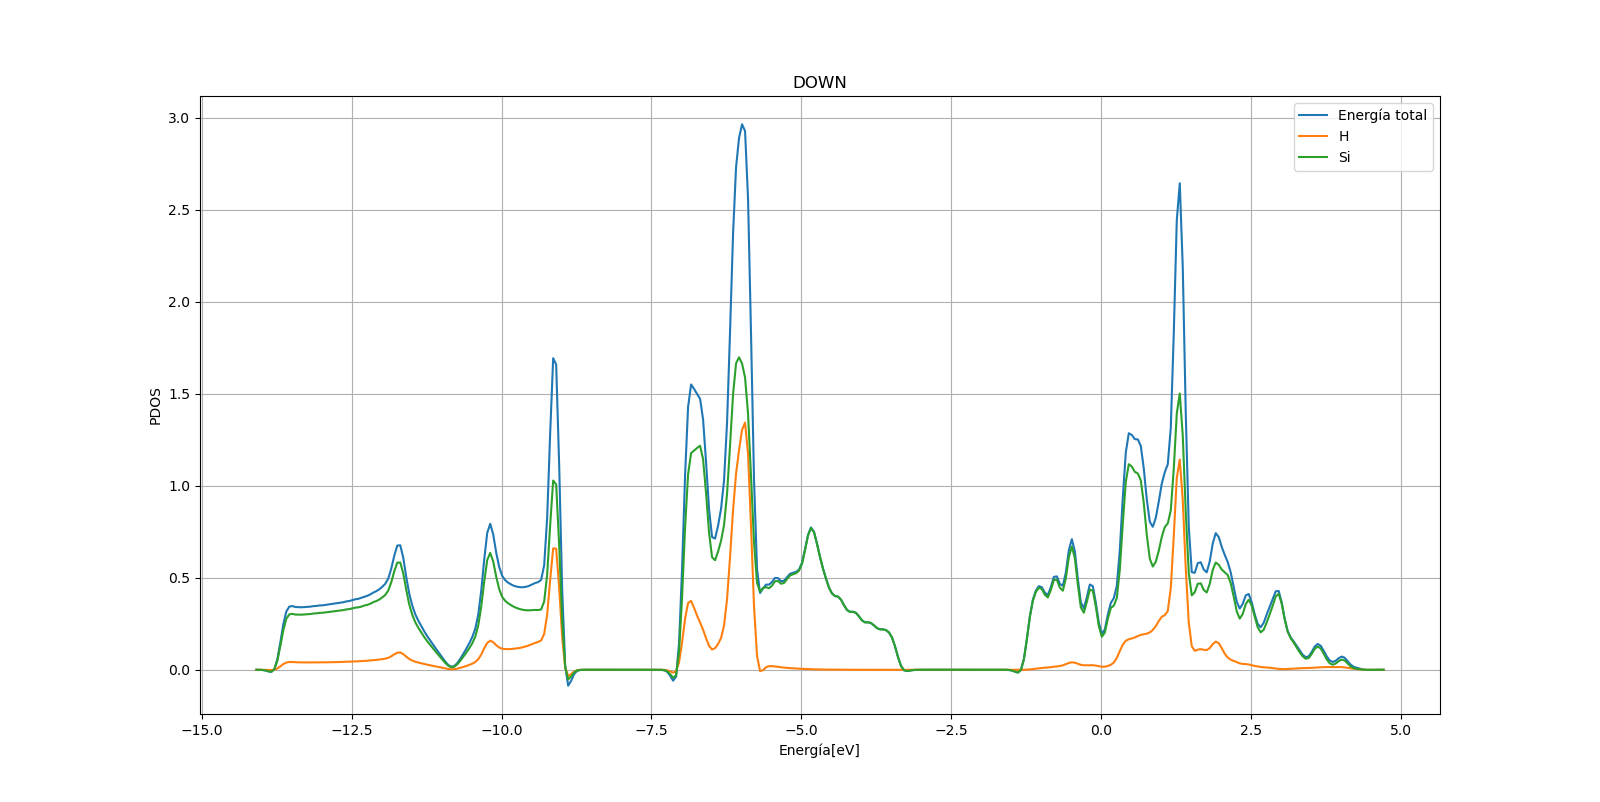
\includegraphics[scale=0.3]{images_silicano/Densidad_estados_con_spin_down_elementos.png}
        \caption{Gráfica que nos muestra la densidad de estados por elemento, sin considerar el spin. [DOWN]}
    \end{figure}    
\end{frame}